\section{Architektur}

    Unabhängig des verwendeten p2p Übertragungsmediums soll eine Schnittstelle in Form eines auf Requests antwortenden Servers zur Verfügung stehen.
	Weit verbreitet ist in diesem Rahmen HTTP als Grundlage für REST und SOAP um einen Webservice anbieten zu können, auch über Proxies und Firewalls hinweg. Für einen p2p Schnittstelle sind solche Vorteile natürlich unerheblich, da die Schnittstelle nicht über eine entfernte Verbindung nutzbar ist, jedoch ist es dennoch von Vorteil, sich darauf festzulegen, eine solche Protokolldefinition zu nutzen, um zur Schnittstellenanbindung und -Implementierung weit verbreitete und damit stabile Bibliotheken nutzen zu können.
    Da sich eine REST Schnittstelle durch die Pakete zinc\footnote{https://github.com/zweidenker/zinc/} und OpenAPI\footnote{https://github.com/zweidenker/openapi} leicht in pharo definieren lässt, bietet es sich an, diese fertigen Serverkomponenten auch zu nutzen.
    Um REST als Schnittstelle jedoch nutzen zu können muss der genutzte Kommunikationskanal HTTP übertragen können. Da jede der vorgestellten Schnittstellen Bytes oder Strings
    übertragen kann, stellen die Übertragungsmedien kein Problem dar, jedoch muss der REST-Server im Falle von Bluetooth, NFC und USB die HTTP-String Repräsentationen zur Verfügung stellen können,
    ohne sie über eine TCP/IP-Netzwerkschnittstelle zu versenden. Ebenso muss der Client die HTTP-Nachrichten korrekt verarbeiten können.
    Da die meisten Bibliotheken an den TCP/IP-Stack von Android gekoppelt sind, um einen gekapselten HTTP-Client anbieten zu können, ist es nicht immer möglich eine String-Repräsentation des zu tätigenden Aufrufs zu erhalten oder an die Bibliothek zu übergeben.
    Die OkHttp Bibliothek\footnote{https://github.com/square/okhttp} sollte diese Probleme jedoch umgehen können, da Netzwerk Aufrufe durch eine Kette von Interceptoren gereicht werden und der RealNetworkInterceptor,
    welcher sich als Letztes in dieser Kette befindet, überschrieben werden kann.
	Im folgenden wird jedoch nur noch, WiFi Direct und damit eine TCP/IP-Implementierung betrachtet.
	
    Um die Schnittstelle einfach warten und erweitern zu können, wird sie als JSONSchema über OpenApi dokumentiert und dem Client zur Verfügung gestellt.
    JSONSchema ist eine Spezifikation, die es erlaubt JSON menschenlesbar zu beschreiben und ebenso durch Maschienenlesbarkeit zu validieren. \footnote{https://json-schema.org/} In Kombination mit OpenAPI ermöglicht es so, eine gesamte Schnittstelle zu beschreiben und als einzelnen Server-Aufruf anzubieten. \footnote {https://swagger.io/docs/specification/about/} Dadurch wird so die Dokumentation der Schnittstelle an die Implementierung gekoppelt. Um die Dokumentationsarbeit so gering wie möglich zu halten, wird OpenAPI so genutzt, dass die Dokumentation direkt aus der Implementierung generiert wird. Dadurch sind Abweichungen der Dokumentation von der Implementierung ausgeschlossen.

	\subsection{Funktionsanforderungen}

    Die zu definierende Schnittstelle muss folgende Funktionalitäten anbieten:
    \begin{itemize}
        \item Eine Auflistung der verfügbaren Netzwerkschnittstellen sollte ähnlich zu {\it ip link show} zur Verfügung stehen, um die ID der gewünschten Schnittstelle für die nächsten Aufrufe herauszufinden.
        \item Pro Netzwerkschnittstelle soll eine Liste der aktuell erreichbaren Netzwerke ausgegeben werden können.
        \item Eine Netzwerkschnittstelle muss konfigurierbar sein, um sich mit einem Netzwerk verbinden zu können. Dazu zählt, eine Liste der bestehenden Konfigurationen zu erhalten, eine Konfiguration auszuwählen, eine einzelne Konfiguration abzufragen und neue Konfigurationen anlegen zu können. Für ein WiFi- Netzwerk muss eine Konfiguration aus der gesendeten ID des Netzwerks und einem optionalem Netzwerkschlüssel bestehen, da alle verbleibenden Informationen über das Netzwerk vom Broadcast des Access Points des zu verbindenden Netzwerks erhalten werden kann.
        Passwörter sollten jedoch aus Sicherheitsgründen nicht wieder über die Schnittstelle ausgegeben werden.
        
        \item Die Spezifikation der Schnittstelle soll als Aufruf der Schnittstelle zur Verfügung stehen, sodass sie leicht nutzbar ist.
    \end{itemize}
    
    \subsection{P2P Anbindung}

	Die REST Schnittstelle muss jedoch über eine Verbindung zur Verfügung gestellt werden, über die unter Umständen nicht direkt die Sockets des Gerätes, auf dem der REST-Server sich befindet, angesprochen werden können. In diesem Fall ist generell ein Eingriff in den IP-Protokollstack nach dem OSI-Referenzmodell mindestens ab der Transportschicht nötig. Im Rahmen der P2P Anbindung muss das Gerät, auf welchem die Konfiguration der Netzwerkschnittstellen möglich sein soll, zusätzlich sich anderen Geräten in der Nähe zu erkennen geben durch ein Beacon-Signal (p2p-Serivce-Discovery), das ähnlich zu DNS Service Discovery ausgesendet wird um eine Zero-Konfiguration Nutzung zu ermöglichen.\footnote{DNS ZERO CONF DOKUMENT REFERENZIEREN.}
	
	\begin{figure}[ht]
	\centering
    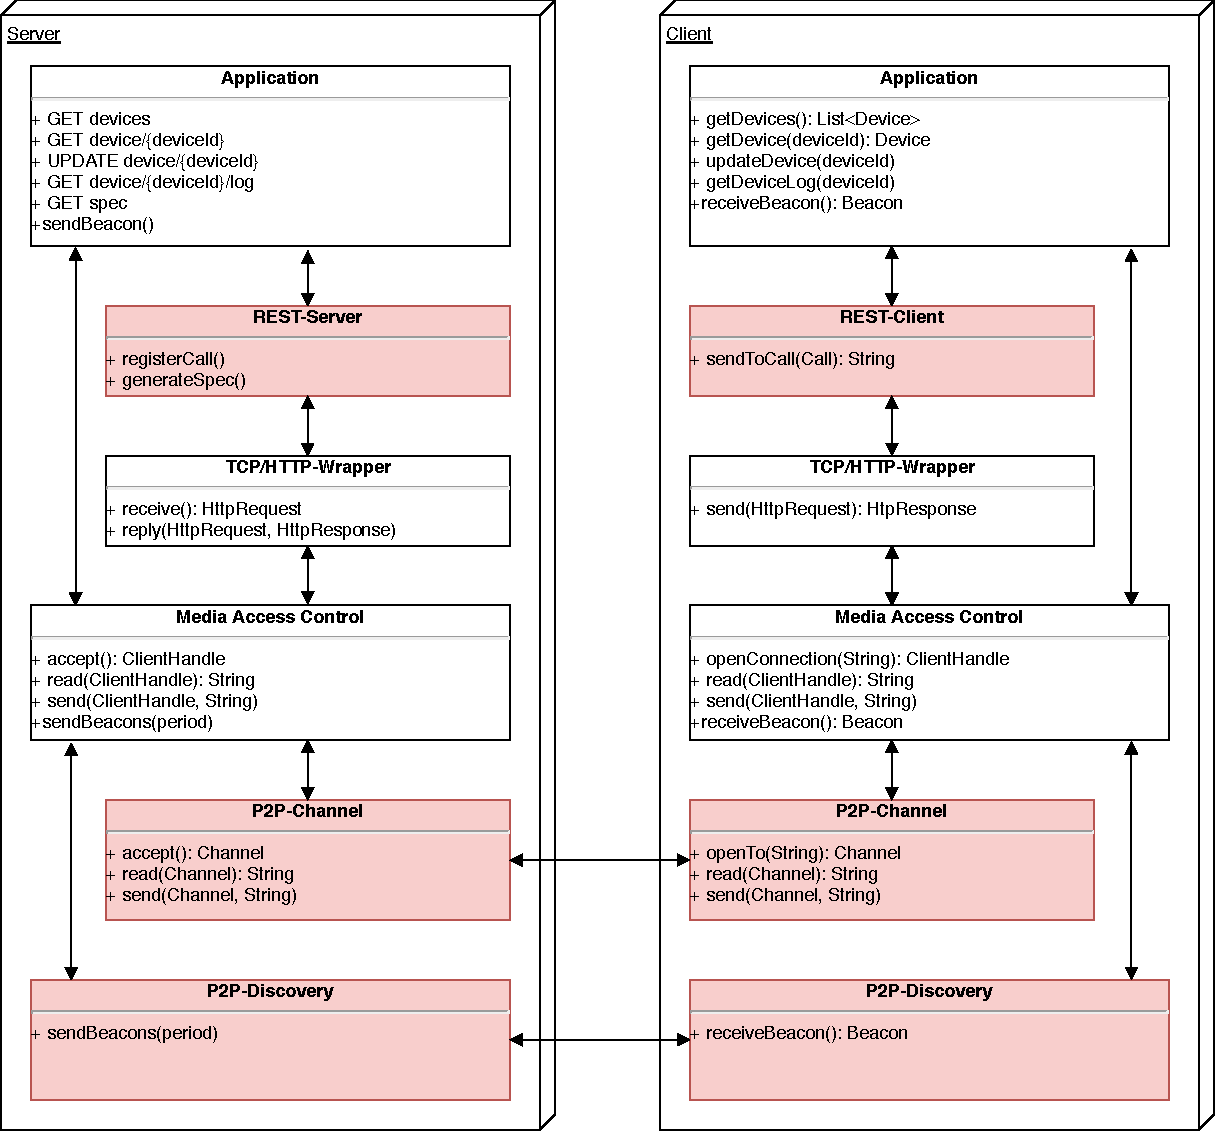
\includegraphics[width=1.0\textwidth]{IOT-Connectivity-Protocol-Stack}
    \caption{Zu sehen sind die Schnittstellen, die nötig sind, um die Client-Server Anwendung über p2p nutzen zu können. Hierbei stehen alle rot hinterlegten Schnittstellen bereits zur Verfügung. Wenn die genutzte p2p Schnittstelle es nicht erlaubt, TCP/HTTP Pakete an die Ports einer Netzwerkschnittstelle des Servers zu senden, muss ein TCP/HTTP-Wrapper erstellt werden. Andernfalls besteht die Implementierung aus einem gewöhnlichem REST-Client/Server-Paar. Getrennt davon muss jedoch auch innerhalb der Anwendung die p2p-Service-Discovery angebunden werden. }
    \label{protocol_stack}
\end{figure}

    \figurename \ref{protocol_stack} zeigt, welche Elemente existieren müssen, um die Serveranwendung als REST-Server Clientgeräten zur Verfügung zu stellen. Größtenteils stehen diese Elemente bereits durch das Betriebssystem und Bibliotheken bereit, jedoch müssen diese gegebenenfalls mit einem TCP/HTTP-Wrapper verbunden werden. Dieser muss dazu in der Lage sein, den REST-Server mit HTTP-Anfragen ansprechen zu können und auf der anderen Seite diese HTTP-Anfragen und Antworten in den p2p-Channel speisen. Dieser Wrapper ist dann sowohl auf Client- sowie auf Server-Seite nötig. 